\documentclass[11pt]{article}
\usepackage[margin=0.85in]{geometry}
\usepackage[T1]{fontenc}
\usepackage{lmodern}
\usepackage{xcolor}
\usepackage{listings}
\usepackage{booktabs}
\usepackage{amsmath,amssymb}
\usepackage{hyperref}
\usepackage{enumitem}
\usepackage{tikz}
\usetikzlibrary{arrows.meta,positioning}
\hypersetup{colorlinks=true,linkcolor=blue!55!black,urlcolor=blue!55!black}
\definecolor{codebg}{HTML}{F5F7FA}
\definecolor{codeblue}{HTML}{2457A6}
\definecolor{codegreen}{HTML}{287A48}
\definecolor{codestring}{HTML}{A33A20}
\lstdefinestyle{python}{language=Python,basicstyle=\ttfamily\small,keywordstyle=\color{codeblue}\bfseries,commentstyle=\color{codegreen}\itshape,stringstyle=\color{codestring},showstringspaces=false,breaklines=true,frame=single,rulecolor=\color{black!18},backgroundcolor=\color{codebg},numbers=left,numberstyle=\tiny\color{black!45},numbersep=8pt,upquote=true,columns=fullflexible}
\title{LLM-Elicited Preferences in an EDSL School-Choice Machine}
\author{School-choice deferred-acceptance pilot}
\date{October 11, 2026}
\begin{document}
\maketitle

\begin{abstract}
This pilot connects LLM-elicited student preferences to a declarative EDSL implementation of many-to-one deferred acceptance. Twelve student personas rank four schools with three seats each. The same elicited preference profile and the same seeded school priorities are used in student-proposing and school-proposing runs. Both outcomes are complete, capacity-feasible, and stable. Student-proposing DA gives all twelve personas their first choice; school-proposing DA gives seven their first choice and has mean student rank 1.75. This is a small mechanism demonstration: it tests the LLM-to-Machine data path and the proposer-side distinction, not the validity of LLM-generated preferences as a model of real families.
\end{abstract}

\section{Question and design}
Can EDSL's shared-state Machine represent the state transitions of school-choice deferred acceptance while receiving preferences elicited from LLM interviews? This pilot uses a deliberately small balanced market: twelve students, four schools, and capacity three at every school. Each student receives a short persona describing location and educational interests. Each school has a short catalog description. One LLM ranking response supplies each student's complete strict ranking of the four schools.

The preference survey is run locally from the project process through the configured OpenAI provider using EDSL's \texttt{disable\_remote\_inference=True}. The model is \texttt{gpt-4o-mini}, temperature 0.2. “Locally” here describes where EDSL executes the interview orchestration and handles credentials; the model inference itself is served by the configured provider. No local inference server is involved.

School priorities are strict random orderings generated from seed 42017. The two mechanism runs consume the exact same LLM preference profile and priority lists. Only the proposer side changes. The complete inputs, rankings, proposal logs, outcomes, and summary metrics are saved in \texttt{preferences.json} and \texttt{results.json} beside this report.

\section{Formal market and stability}
Let $S$ be the finite student set and $C$ the school set. School $c$ has capacity $q_c=3$. Each student $s$ has a strict preference order $\succ_s$ over all schools, and each school $c$ has a strict priority order $\succ_c$ over all students. A matching $\mu$ assigns each student to one school and no school more than its capacity.

A pair $(s,c)$ blocks $\mu$ when student $s$ prefers $c$ to their assignment and either $c$ has an unfilled seat or $c$ prioritizes $s$ over at least one currently assigned student:
\[
  c \succ_s \mu(s) \quad\text{and}\quad
  \bigl(|\mu(c)|<q_c\;\;\text{or}\;\;\exists s'\in\mu(c):s\succ_c s'\bigr).
\]
A matching is stable if it has no blocking pair.

In student-proposing DA, each unheld student proposes to their most-preferred school not yet approached. Each school holds its highest-priority applicants up to capacity and rejects the remainder. In school-proposing DA, each school with an open seat proposes to its highest-priority student not yet approached. Each student holds their favorite offer to date; a rejected school advances down its priority list. Strict preferences, complete lists, finite participants, and no repeated proposals imply termination.

\section{Machine state and embedded loop}
The EDSL Machine stores the market instance as constants: participants, capacities, preferences, school priorities, and rank maps. Its single mutable field, \texttt{allocation}, is a typed record containing the proposal queue, student assignments, tentative school holds, both proposer cursor maps, the proposal log, and a completion flag. The full procedure is an EDSL \texttt{iterate} expression in \texttt{close\_effects}. In each iteration, a pure expression reads the current allocation, selects the next eligible proposer, forms the proposal, returns a complete next allocation record, and records the outcome. The bounded loop terminates when its declared queue or active-school condition is true. No named Python callback is used (\texttt{algorithms=()}).

\begin{figure}[h]
\centering
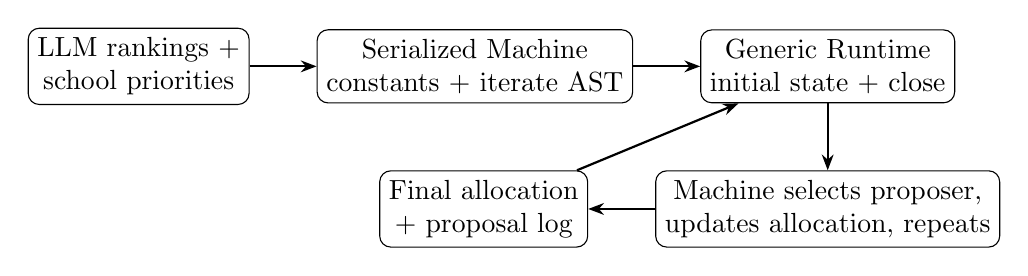
\begin{tikzpicture}[node distance=.85cm,every node/.style={draw,rounded corners,align=center,minimum width=2.5cm,minimum height=.7cm},arr/.style={-{Stealth[length=2mm]},thick}]
\node (profile) {LLM rankings +\\school priorities};
\node[right=of profile] (machine) {Serialized Machine\\constants + iterate AST};
\node[right=of machine] (runtime) {Generic Runtime\\initial state + close};
\node[below=of runtime] (loop) {Machine selects proposer,\\updates allocation, repeats};
\node[left=of loop] (output) {Final allocation\\+ proposal log};
\draw[arr] (profile)--(machine); \draw[arr] (machine)--(runtime); \draw[arr] (runtime)--(loop); \draw[arr] (loop)--(output); \draw[arr] (output)--(runtime);
\end{tikzpicture}
\caption{The matching loop is in the serialized Machine; Python invokes only the generic Runtime lifecycle.}
\end{figure}

The student-proposing loop removes the first student from its queue, selects that student's next ranked school, sorts the school's incumbents plus new applicant by priority, retains up to capacity, requeues rejected students, and advances the student's cursor. The school-proposing loop selects the first school with an open seat and an untried student, makes that offer, lets the student keep their preferred school, and advances the school's cursor. Each loop has a finite explicit bound. The close transition computes the final allocation atomically; intermediate states are preserved as proposal-log entries rather than committed one by one.

\section{Run procedure}
First, the survey defines one \texttt{QuestionRank} with all four school IDs as options and requires a complete ranking. Second, twelve persona agents answer with their individual profile inserted into the prompt. Third, each response is validated as a permutation of all four schools and saved. Finally, each proposer-side Machine embeds that saved preference profile and the seeded school priorities. The generic runner initializes the Runtime and invokes the standard close operation; it has no school-choice-specific proposer loop.

The core local-execution setting is:
\begin{lstlisting}[style=python]
results = (survey.by(agents)
    .by(Model(model_name, service_name="openai", temperature=0.2))
    .run(cache=False, disable_remote_cache=True,
         disable_remote_inference=True, max_concurrency=4,
         stop_on_exceptions=True))
\end{lstlisting}

The same saved preferences are passed to both Machine definitions:
\begin{lstlisting}[style=python]
machine = build_machine(seed, proposer_side, preferences)
runtime = Runtime()
state = runtime.initial_state(machine)
final = runtime.close_result(machine, state)
\end{lstlisting}

\section{Results}
\begin{center}
\begin{tabular}{lrr}
\toprule
Outcome & Student-proposing & School-proposing \\
\midrule
First-choice assignments & 12/12 & 7/12 \\
Mean student rank (1 = best) & 1.00 & 1.75 \\
Proposal transitions & 12 & 22 \\
Blocking pairs & 0 & 0 \\
Seats filled & 12/12 & 12/12 \\
\bottomrule
\end{tabular}
\end{center}

Student-proposing DA produces the student-optimal stable matching for this fixed market, so it is weakly better for every student than any other stable matching, including the school-proposing outcome. In this particular preference profile, all students receive their first-ranked school in the student-proposing outcome. In school-proposing DA, five students receive a lower-ranked school: four are assigned their third choice and one their second choice. Both outcomes satisfy capacities and have no blocking pairs.

The unusually clean student-side outcome is a property of this specific elicited ranking profile together with the priority draws: every student receives the school at the top of their list, and each school receives exactly three first-choice applicants. It should not be read as a general property of school choice or of this prompt. Repeated LLM interviews, alternative seeds, and human preference data would be needed to characterize the distribution of outcomes.

The Machine logged 12 student proposals and 22 school proposals. This difference reflects distinct proposal protocols and does not by itself indicate computational performance. The same saved rankings are embedded in both serialized Machines; each Machine includes its proposer selection and repeat-until loop in its close effect.

\section{Interpretation and limitations}
This pilot demonstrates an end-to-end integration: a structured EDSL ranking question produces machine-readable strict preferences, the preferences are validated and persisted, two serialized Machine configurations run against the same market, and independently checked outcomes are stable. It also makes proposer-side consequences visible in a compact, auditable example.

It does not establish that LLM personas behave like real students or families. Persona descriptions are authored inputs, not sampled people; a single completion per persona cannot measure response variability; the model's internal assumptions may affect rankings; and the priorities are seeded synthetic rankings rather than an institutional admissions policy. The result is a software and mechanism pilot, not an empirical policy evaluation. A stronger next study would collect multiple independent ranking draws per persona, vary model and prompt, evaluate sensitivity to persona and school-description wording, and report outcome distributions across many priority seeds.

\appendix
\section{Reproduction and artifacts}
From the repository root, run the LLM pilot with:
\begin{lstlisting}[style=python]
PYTHONPATH=edsl_replication/studies/school_choice_deferred_acceptance \\
  python3 edsl_replication/studies/school_choice_deferred_acceptance/llm_pilot.py
\end{lstlisting}
The command requires the provider key to be configured in the local environment. It writes preference and outcome JSON to \texttt{pilot\_llm\_01/}. To rerun only the deterministic matching step on the saved profile, pass \texttt{--reuse-preferences}. The EDSL CAS object store is directed into \texttt{pilot\_llm\_01/edsl\_objects/} so the runner's local result persistence remains inside the study artifact.

\begin{itemize}[leftmargin=*]
\item \texttt{machine\_definition.py}: Machine constants, typed allocation, and bounded EDSL loops.
\item \texttt{run\_pilot.py}: generic Runtime initialization and close, followed by independent capacity/stability checks.
\item \texttt{llm\_pilot.py}: persona survey, ranking validation, local EDSL run, and LLM-profile comparison.
\item \texttt{preferences.json}: the 12 elicited strict rankings.
\item \texttt{results.json}: both Machine outcomes, priorities, event logs, and metrics.
\end{itemize}

See the companion \texttt{machine\_technical\_note.pdf} for syntax-highlighted source excerpts and the complete details of the serialized loop, state record, step bounds, and generic Runtime call.

\end{document}
